\documentclass{article}
\linespread{1.25}

\usepackage{pgfplots}
\pgfplotsset{compat=1.18}

\usepackage[top=2cm, right=2cm, left=2cm]{geometry}
\usepackage{graphicx}
\usepackage[section]{placeins}
\usepackage[hidelinks, urlcolor=blue]{hyperref}
\usepackage{float}
\usepackage[perpage, stable]{footmisc}
\usepackage{amsmath}
\usepackage{titling}



% Commands
\newcommand{\column}[1]{\textit{#1}}


% Custom title page setup
\makeatletter
\def\maketitle{
	\begin{titlepage}
		\begin{center}
			\vspace*{2cm}
			
			{\Large\bfseries Machine Learning Course\par}
			\vspace{2cm}
			
			{\Huge\bfseries Linear Regression Assignment Solution\par}
			\vspace{3cm}
			
			{\large\bfseries Professor:\par}
			{\large Dr. Mahdi Eftekhari\par}
			\vspace{1.5cm}
			
			{\large\bfseries Author:\par}
			{\large Amirhossein Abolhassani\par}
			\vspace{2cm}
			
			\vfill  % pushes the date to bottom
			
			{\large\bfseries Fall 2024}
			
		\end{center}
	\end{titlepage}
	\setcounter{page}{1}
}
\makeatother

\begin{document}
	\maketitle	
	\section*{Question 1}
	\subsection{Scatter Plot}
	\begin{center}
		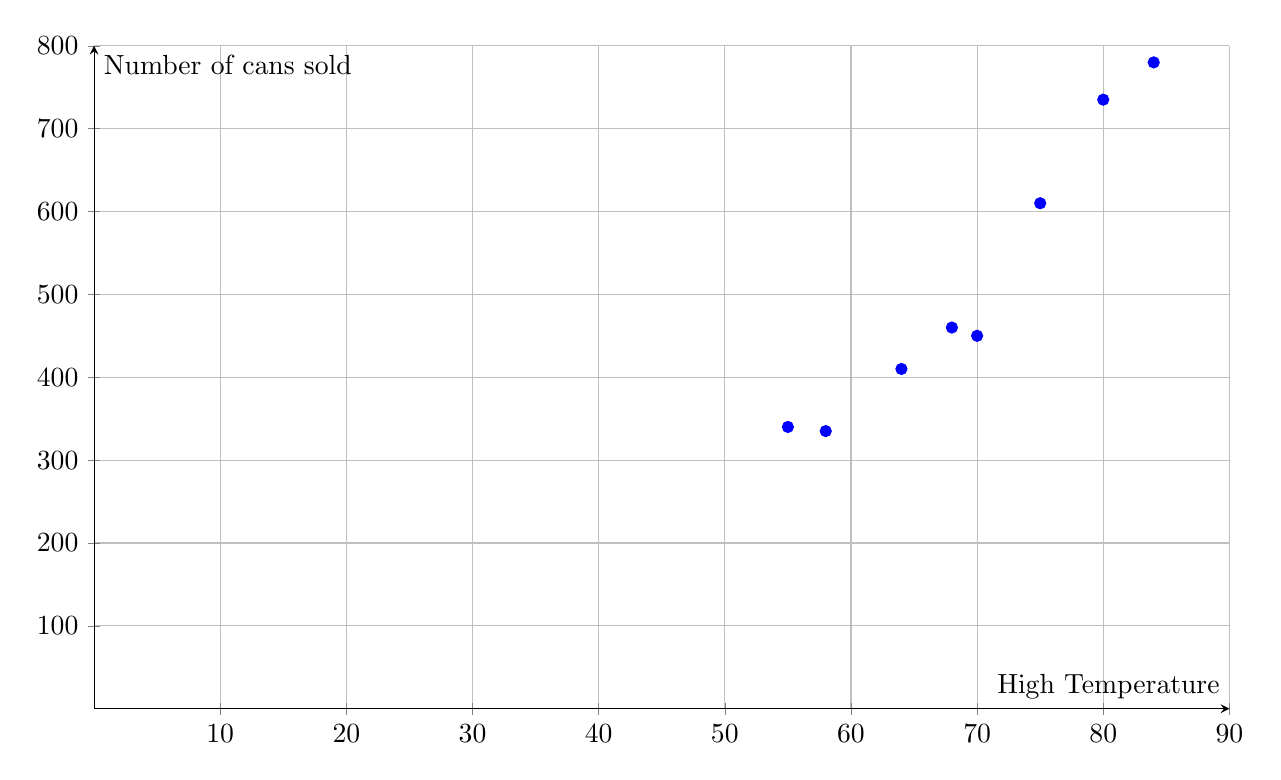
\begin{tikzpicture}
			\begin{axis}[
				xlabel={High Temperature},
				ylabel={Number of cans sold},
				grid=major,
				width=16cm,
				height=10cm,
				xmin=0, xmax=90,  % Set the x-axis range
				ymin=0, ymax=800,  % Set the y-axis range
				axis lines=middle, % Place the axes at the origin
				]
				\addplot[
				only marks,
				mark=*,
				color=blue,
				] coordinates {
					(55, 340)
					(58, 335)
					(64, 410)
					(68, 460)
					(70, 450)
					(75, 610)
					(80, 735)
					(84, 780)
				};
			\end{axis}
		\end{tikzpicture}
	\end{center}
	\subsection{Equation and Plot of Linear Regression for the Data}
	To obtain the regression parameters:
	\begin{flalign*}
		\theta  & = (X^TX)^{-1}X^T\vec{y}\\
		& = \left(\begin{pmatrix}
			1&1&1&1&1&1&1&1 \\
			55& 58& 64& 68& 70& 75& 80 & 84
		\end{pmatrix}
		\begin{pmatrix}
			1 & 55\\
			1 & 58\\
			1 & 64\\
			1 & 68\\
			1 & 70\\
			1 & 75\\
			1 & 80\\
			1 & 84
		\end{pmatrix}\right)^{-1}
		\begin{pmatrix}
			1&1&1&1&1&1&1&1 \\
			55& 58& 64& 68& 70& 75& 80 & 84
		\end{pmatrix}
		\begin{pmatrix}
			340\\
			335\\
			410\\
			460\\
			450\\
			610\\
			735\\
			780
		\end{pmatrix}\\
		& = \begin{pmatrix}
			8 & 554\\
			554 & 39090
		\end{pmatrix}^{-1}
		\begin{pmatrix}
			4120 \\
			297220
		\end{pmatrix}\\
		& = \begin{pmatrix}
			6.73501034 & -0.0954514128\\
			-0.0954514128 & 0.00137835975
		\end{pmatrix}
		\begin{pmatrix}
			4120 \\
			297220
		\end{pmatrix}\\
		& = \begin{pmatrix}
			-621.82632667\\
			16.41626465
		\end{pmatrix}
	\end{flalign*}
	Thus, the linear equation is:
	\[ y = -621.82632667 + 16.41626465 x \]
	And plotted as:
	\begin{center}
		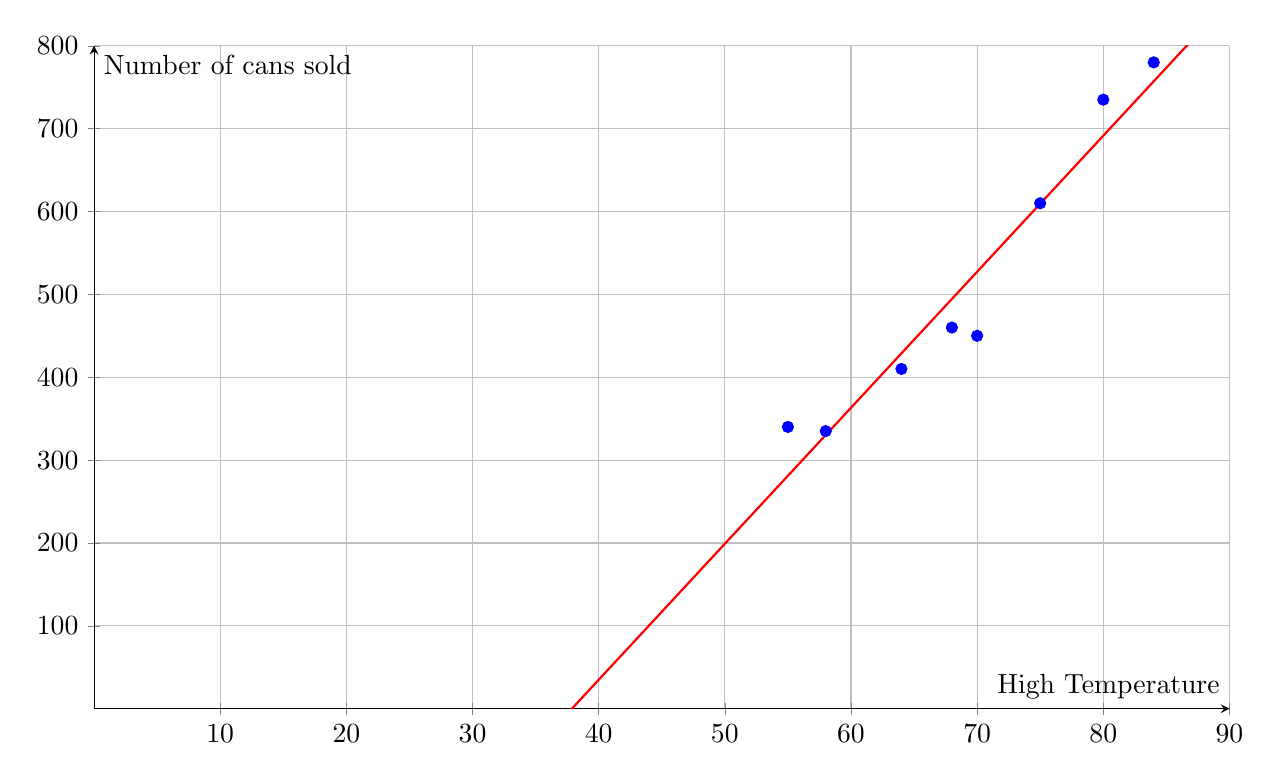
\begin{tikzpicture}
			\begin{axis}[
				xlabel={High Temperature},
				ylabel={Number of cans sold},
				grid=major,
				width=16cm,
				height=10cm,
				xmin=0, xmax=90,  % Set the x-axis range
				ymin=0, ymax=800,  % Set the y-axis range
				axis lines=middle, % Place the axes at the origin
				]
				\addplot[
				only marks,
				mark=*,
				color=blue,
				] coordinates {
					(55, 340)
					(58, 335)
					(64, 410)
					(68, 460)
					(70, 450)
					(75, 610)
					(80, 735)
					(84, 780)
				};
				
				\addplot[
				domain=0:100, % Range for x-axis
				samples=2,  % Number of points for smoothness
				thick,
				color=red,
				] {-621.82632667 + 16.41626465*x}; % Replace with your line equation
			\end{axis}
		\end{tikzpicture}
	\end{center}
	\subsection{Prediction with the Obtained Model}
	For \( x = 95^{\circ} F \):
	\begin{flalign*}
		y & = \begin{pmatrix}
			1 & x
		\end{pmatrix}
		\begin{pmatrix}
			-621.82632667\\
			16.41626465
		\end{pmatrix}\\
		& = 937.71881508
	\end{flalign*}
	\subsection{Inverse Model Prediction}
	The equation is:
	\[ \theta_0 + \theta_1 x = 95 \rightarrow x = \frac{95 - \theta_0}{\theta_1} \]
	From which the temperature is calculated:
	\[ x = \frac{95 - (-621.82632667)}{16.41626465} \rightarrow x = 43.6656 \]
	\section*{Question 2}
	\subsection{Problem 1}
	The problem is Classification because the output is discrete.
	\subsection{Problem 2}
	The problem is Regression because we aim to examine the impact of features on a continuous target variable.
	\subsection{Problem 3}
	The problem is Classification because we predict class 0 or 1 for the specified disease.
	\section*{Question 3}
	The second hyperparameter setting is chosen because it has the lowest training and test errors, with zero difference between them, indicating no overfitting.
	\section*{Question 4}
	Here, the independent variable is \( y \), and the dependent variable is \( x \). Thus, we need to find the weights for the equation:
	\[ x = \theta_0 + \theta_1 y \]
	We know:
	\begin{flalign*}
		\theta  & = (\vec{y}^T\vec{y})^{-1}\vec{y}^T\vec{x}\\
		& = \begin{pmatrix}
			1.09549706\\
			0.92451599
		\end{pmatrix}		
	\end{flalign*}
	The final model is:
	\[ x = 1.09549706 + 0.92451599 y \]
\end{document}